\setRL
\clearpage

\def \MemBio {\Mempath /MembraneBio}

\section{
چکیده
}
این فصل با مقدمه‌ای از نقش غشای زیستی در سلول شروع شده‌است (بخش
\ref{sec:memBioIntro}).
 سپس، مرور کوتاهی بر تارخچه‌ی تحقیقات انجام شده در جهت کشف و بررسی ساختار غشای سلول‌های زنده در قرن‌های ۱۹ و ۲۰ میلادی ارايه شده‌است (بخش
\ref{sec:memBioHistory}).
در ادامه، در مورد ساختار واحد‌های تشکیل دهنده‌ی غشا بحث شده (
\ref{sec:memBioSelfAssembily}
تا
\ref{sec:memBioFluidity})
 و در نهایت در مورد چیدمان غشای هسته یا بسته‌ی هسته توضیح داده شده‌است (بخش
\ref{sec:nuclearenvelope}).
 
 
\section{\label{sec:memBioIntro}
مقدمه
}
\setRL
%\pagenumbering{arabic} 


%\section{\label{sec:cellmembrane}
%غشای سلولی
%}
\section{
مقدمه
}
\begin{figure}[h]
\begin{center}
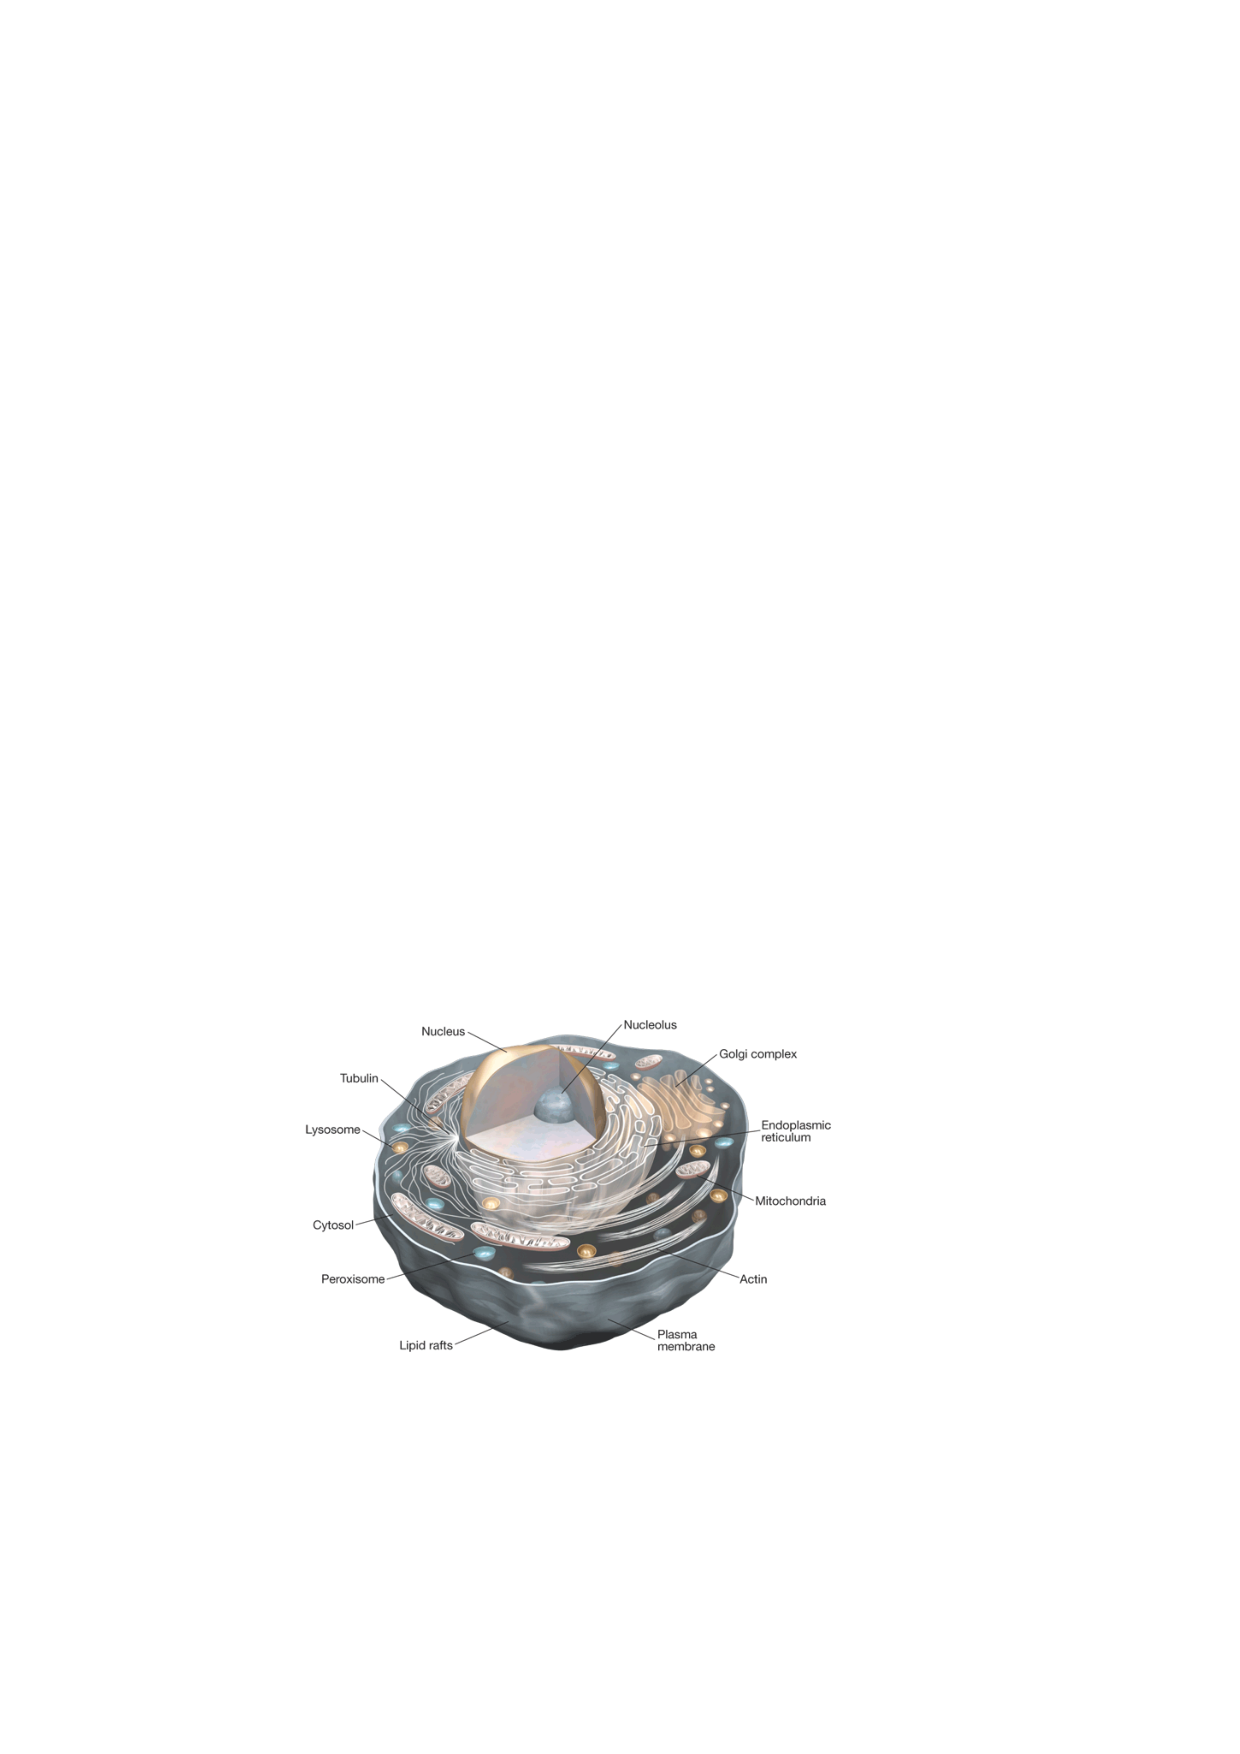
\includegraphics[width=6in]{\MemBio /Pics/CellParts}
\caption{
شکل طراحی شده از سلول پستانداران که غشا و اعضای سلول را نشان می‌دهد
\cite{CellParts}.
}
\label{fig:cellparts}
\end{center}
\end{figure}

مهم‌ترین نقش غشاهای زیستی ایجاد یک دیوار یا مانع برای مشخص کردن مرز داخل و خارج سلول است که نیاز اولیه‌ی وجود حیات به حساب می‌آید
\cite{Boyle2008Biology}.
 علاوه بر در-بر-گرفتنِ تمام اعضای یک سلول، در سلول‌های هسته‌دار، غشای هسته اورگان‌های خیلی مهم سلول را نیز در خود جا داده و محافظت می‌کند (شکل
\ref{fig:cellparts}). به عنوان مرز سلول با دینای خارج، غشا نقش مهمی در مدیریتِ نقل و انتقال مواد بین سلول و محیط پرامون دارد. درون غشا پروتئین‌ها، لیگاند‌ها
\LTRfootnote{ligand}،
و ملکول‌های درشت خیلی زیادی وجود دارد که در طیف‌ گسترده‌ای از فرآیندها نقش دارند. برای مثال غشا نقل و انتقال یون‌ها به درون و خارج سلول را از طریق کانال‌های پروتئینی مدیریت می‌کند
\cite{NEHER1976ProteinChannel}،
نسبت به تغییر فشار اُسمزی محیط واکنش نشان می‌دهد
\cite{Perozo2006Osmotic,Vasquez2009Osmotic,Haswell2011Osmotic}،
و همچنین در ساز و کار‌های بزرگ مقیاس مانند تقسیم سلولی، حرکت و جابجایی سلول، و چسبیدن به سطوح نقش دارد.


غشای سلول در خیلی از مسائل مهم پزشکی نیز مطرح می‌شود، مانند نقش آن در انتقال پالس الکتریکی در سلول‌های عصبی هنگام بیهوشی عمومی 
\cite{BioMemBook2007}.
همچنین بیشتر تلاش صنعت داروسازی طراحی داروی مناسب برای اتصال به پروتئین‌های روی سطح غشاست. تقریبا یک سوم پروتئین‌های دروی بدن در غشای سلول قرار دارند که  مورد هدف ۶۰ در صد از داروی‌های موجود در بازار هستند
\cite{DrugDelivery2007}.
 دانش یافته شده از مطالعه‌ی غشا در تکنولوژی‌های مدرن مانند بسته‌بندی و انتقال دارو
\cite{Torchilin2006Drugdelivery}،
ایجاد اتاقک‌های کوچک برای انجام واکنش‌های شیمیایی
\cite{Karlsson2001MemChamber}،
 و ساخت حس‌گرهای زیستی (ترکیب دستگاه‌های الکتریکی با غشا) کاربرد دارد
\cite{MemeElctronics2012}.


\section{\label{sec:memBioHistory}
تاریخچه کوتاه
}
\setRL
%\pagenumbering{arabic} 
\section{
تاریخچه کوتاه
}
حاصل زحمات افراد در قرن ۱۹ و ۲۰ میلادی در راستای پی بردن به ساز و کار واحد‌های سازنده‌ی موجودات زنده، ساخت تصویری با جزئیات زیاد از سلول‌های زنده است. در سال ۱۹۸۵ ارنست اُورتن\LTRfootnote{Ernest Overton}  
سلول‌های گیاهی را در محلول‌های مختلف (قند،‌ الکل، اتر، فنول، و اَسِتُن\LTRfootnote{sugar, alcohols, ether, phenol, and acetone}) قرار داد. مشاهدات وی نشان داد که (تحت اختلاف فشار اسمزی یکسان) محلول‌هایی مانند قند که در آب به راحتی حل می‌شوند نمی‌توانند وارد سلول شوند. در صورتی که محلول‌های دیگری که حل شونده‌ی خوبی در آب نیستند، می‌توانند وارد سلول شوند. او نتیجه گرفت که جنس مرز سلول با سیتوپلاسم درون آن متفاوت است و به احتمال زیاد از ملکول‌های چربی گون تشکیل شده است
\cite{overton1985}.

در سال ۱۹۱۷ اِروین لَنگموئر \LTRfootnote{Irving Langmuir}
 مقاله‌ای چاپ کرد که در آن روشی برای اندازه‌گیری فشار جانبی\LTRfootnote{lateral}
 غشا در سطح مقطع مشترک هوا و آب پیشنهاد داد
 \cite{Langmuir1917}.
 او با استفاده از روش خود نشان داد که غشا در این سطح مقطع مشترک یک تک لایه‌ی ملکول چرب تشکیل می‌دهد و مساحت هر ملکول را 
 $S_{lipid} = 0.7 nm^2$
 گزارش کرد. او همچنین در گزارش خود پیشنهاد داد که غشا از ملکول‌های دوزیست\LTRfootnote{Amphiphiles}
 تشکیل شده. ملکول‌های دوزیست به ملکول‌هایی گفته می‌شود که یک گروه سَر دو قطبی آب‌دوست و یک یا چند دُم هیدروکربنی آب‌گریز داشته باشد. 
 
 با به کارگیری روش اندازه‌گیری لنگموئر، در سال ۱۹۲۵، گُرتِر\LTRfootnote{E. Gorter}
 و گرِندِل\LTRfootnote{F. Grendel}
 نشان دادند که  غشای گلبول‌های قرمز از یک دو-لایه لیپید تشکیل شده
 \cite{Gorter1925}.
 آن‌ها غشای گلبول را در اَسِتُن حل کرده و با روش لنگموئر سطح آن را اندازه‌گیری کردند. سپس این عدد را با مساحت گلبول قرمز خشک شده مقایسه کردند. در آزمایش آن‌ها دو خطا وجود داشت؛ اولین خطا در اینجا بود که اَسِتُن نمی‌تواند تمام ملکول‌های چربی را از گلبول جدا کند، و دوم در اندازه‌گیری مساحت گلبول قرمز بود
 \cite{BiomembranesBook1989,BioMemBook2007}.
 ولی خوشبختانه این دو خطای اندازه‌گیری همدیگر را تکمیل کردند و آن‌ها نسبت این دو عدد را با تقریب خوبی نزدیک به ۲ اندازه‌گیری کردند که با اطلاعات فعلی ما از ساختار  دو-لایه غشای گلبول قرمز سازگار است
 \cite{Edidin2003}.
 
  
 
 
 در سال ۱۹۳۲ (حدود نود سال پیش) کِنِت کول\LTRfootnote{Kenneth Cole}
 تخم جوجه‌تیغی دریایی\LTRfootnote{sea urchin (arbacia) egg} 
را بر سطحی قرار داد و  با کمک یک فیبرِ از جنس طلا به تخم  فشار وارد کرد. با اندازه‌گیری  کشش سطحی و مقایسه‌ی آن با حد تحمل فشار تخم، استدلال کرد که لایه‌ی نازکی که در اطراف سلول وجود دارد تنها از ملکول‌های چربی درست نشده است
 \cite{Cole1932}. 

در دهه‌ی ۱۹۳۰ داوسن\LTRfootnote{H. Davson} 
و دنیِلی\LTRfootnote{J. F. Danielli} 
مدل جدیدی برای غشا پیشنهاد دادند. آن‌ها با آزمایش بر روی غشا‌های مصنوعی و سلولی، دلیل اختلاف در تراوایی دو روی غشا در عبور مواد یونی و دوقطبی را وجود لایه‌ای از پروتئین بر روی غشا توصیف کردند
\cite{Danielli1935}. 
این مدل غشا اولین مدلی بود که به طور عمومی پذیرفته  و تا سال‌ها  در تحقیقات استفاده شد. حتی پس از  پدید آمدن ابزار‌های تصویر‌برداری دقیق، این مدل تنها با کمی تغییر جزئی مواجه شد.

در دهه‌ی ۱۹۵۰ با فرا رسیدن تکنولوژی میکروسکوپ الکترونی، رابرتسون\LTRfootnote{J. D. Robertson}
 اولین تصاویر از غشای سلول را رونمایی کرد. وی با استفاده از روش‌های رنگ آمیزی، وجود لیپید‌ها\LTRfootnote{lipid}
 در غشا را تایید و ضخامت غشای سلولی را بین ۵ تا ۱۰ نانومتر اندازه‌گیری کرد
\cite{ROBERTSON1959aa}.
او همچنین نشان داد که غشای پلاسمایی و تمامی اعضای غشاگون مثل غشای هسته‌ی سلول و غشای دو-لایه میتوکندریا\LTRfootnote{mitochondria}
ساختار مشترکی دارند که مدل داوسن-دنیلی و مشاهدات گُرتِر و گرِندِل را تایید می‌کرد.
همچنین درنتیجه‌ی اندازه‌گیری با میکروسکوپ و پراش اشعه‌ی X ضخامت غشا 
 $5-8nm$
و ضخامت لایه‌ی مرکزی آبگریز آن
 $3-4nm$
گزارش شد
\cite{NelsonBook2004}.
با پیشرفت سریع روش‌های اندازه‌گیری و تصویربرداری بر پایه‌ی تشدید مغناطیسی (مانند تشدید مغناطیسی‌ هسته‌ای یا NMR\LTRfootnote{nuclear magnetic resonance}
و تشدید اسپین الکترون\LTRfootnote{electron spin resonance}) آزمایش‌های زیادی طراحی شد که نشان داد غشا  خواصی شبیه به مایع دارد
\cite{Edidin2003}
و لیپید‌ها می‌توانند بر سطح غشا با ضریب پخش
$D_{lipid}\sim 10^{-8}cm^2/s\approx 10^6S_{lipid}/s$
 حرکت کنند
\cite{NelsonBook2004,Chapman1975}.
همچنین عدم تقارن بین دولایه‌ی غشا تایید شد و برای اولین بار با علامت گذاری پروتئین‌های بر روی دو سطح غشا، حضور پروتئین‌ها در درون غشا نشان داده شد
\cite{Bretscher1973}.



افراد زیادی در تکمیل شدن تصویری که امروزه از غشای سلول وجود دارد نقش داشتند، ولی تصویر مدرن ما از غشاهای سلول‌ها بیشتر بر پایه‌ی مدل غشای مایع موزایکی‌\LTRfootnote{the mosaic fluid model of membranes}
 است که در سال ۱۹۷۲ توسط سینگر\LTRfootnote{Singer}
  و نیکلسون\LTRfootnote{Nicholson}
 ارائه شد
\cite{Singer1972}
(شکل 
\ref{fig:fluidmembranemodel}). بنا بر این مدل، غشا را می‌توان یک مایع همگن دو بعدی وُشکسان از چربی‌ها و کُلِسترول فرض کرد که ماکرو-ملکول‌های پروتئینی به کمک برهمکنش‌های آب‌گریز  بر روی سطح یا درون آن قرار گرفته و کم و بیش آزادانه حرکت می‌کنند (مانند دریای قطب شمال و تکه‌های یخ  شناور در آن).  در نتیجه هیچ نظم بلند بردی در غشا دیده نمی‌شود. 

\begin{figure}[h]
\begin{center}
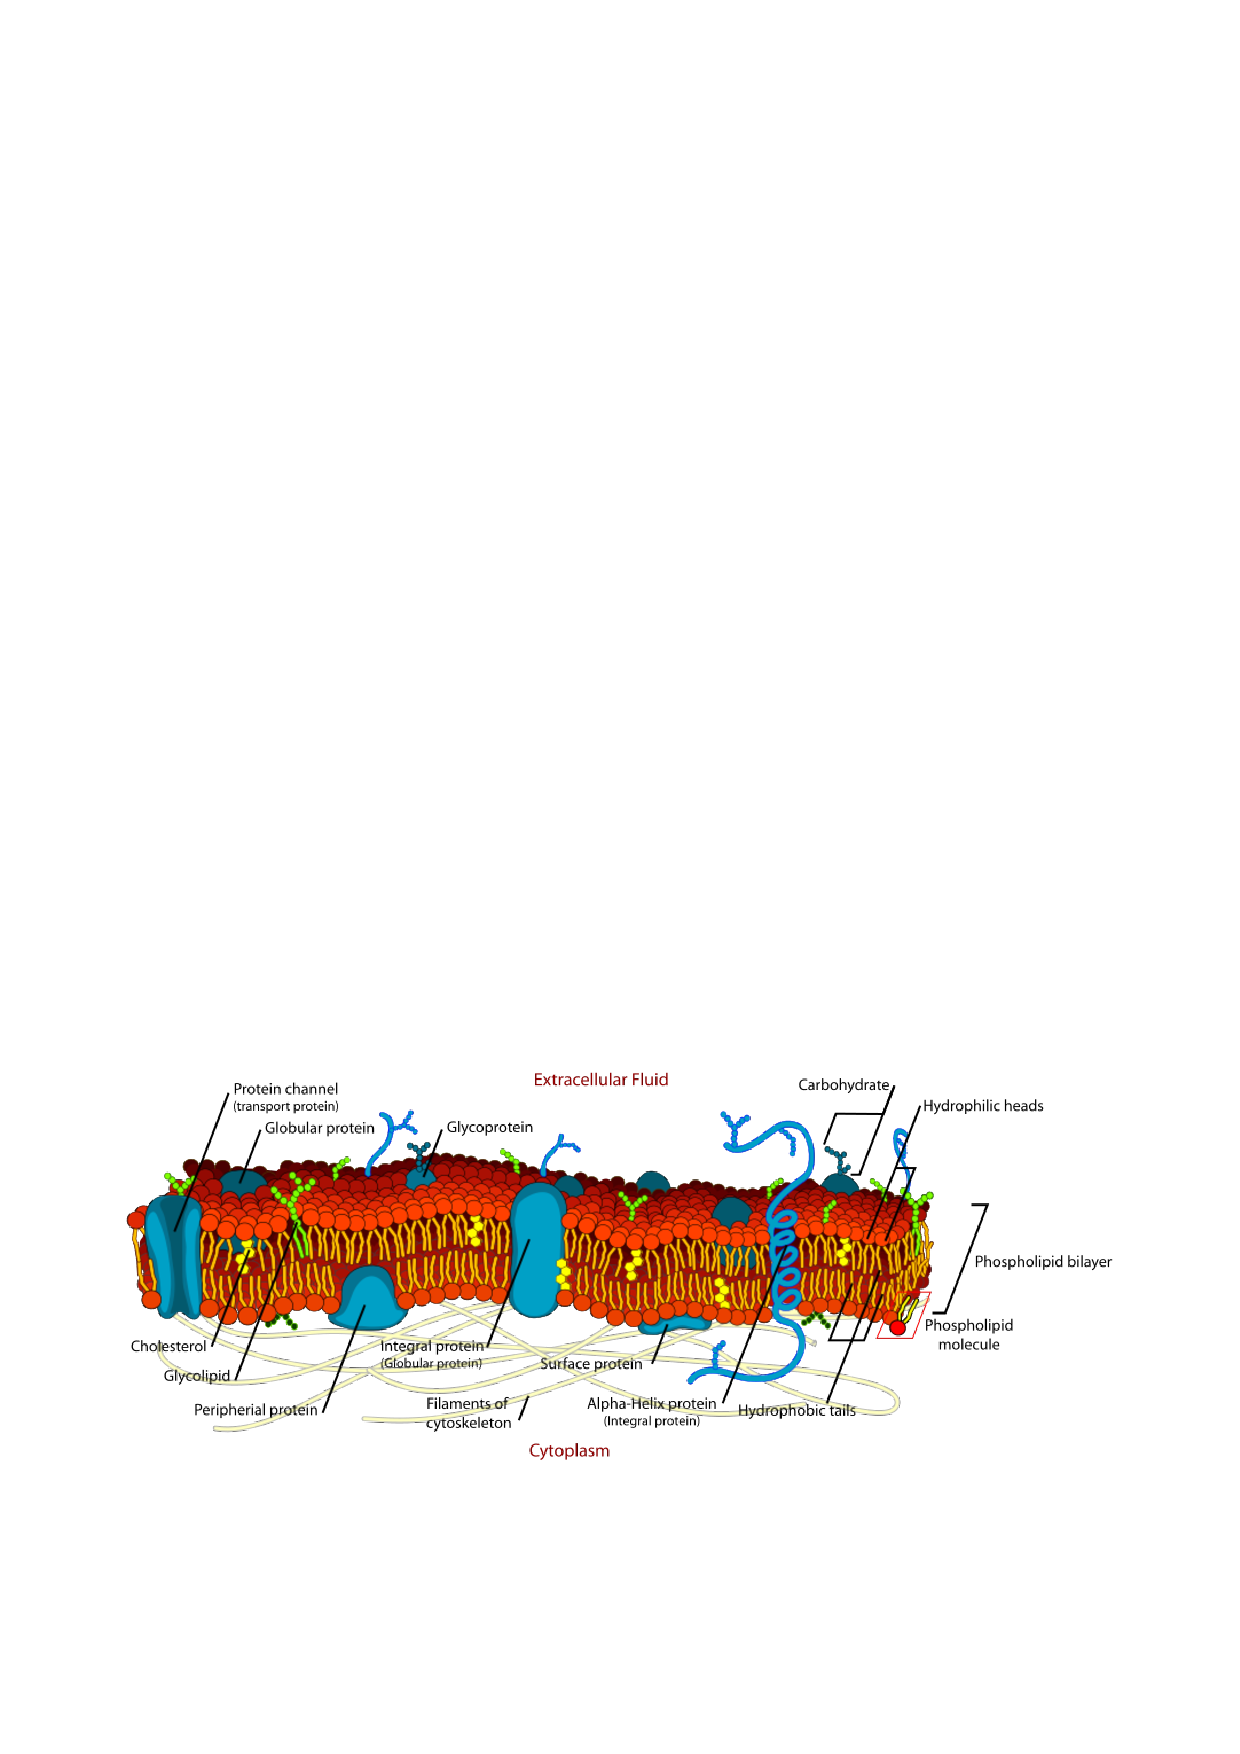
\includegraphics[width=4in]{\MemBio /Pics/Cell_membrane_detailed_diagram}
\caption{
شکل از سایت ویکیپیدیا گرفته شده است
\cite{wikiCellMembrane}. این یک نقاشی از غشا بر اساس مدل غشای مایع موزایکی است. بیشتر غشا از ملکول‌های چربی تشکیل شده ولی پروتئین‌های خیلی زیادی نیز در غشا قرار دارد.  غشا از طریق این پروتئین‌ها به اسکلت سلولی و اجزای دیگر متصل است. دایره‌های قرمز سر آب‌دوست و رشته‌های زرد دُم‌های آب‌گریز لیپید‌ها را نشان می‌دهد.
}
\label{fig:fluidmembranemodel}
\end{center}
\end{figure}


در نتیجه‌ی توسعه‌ی تحقیقات، می‌دانیم غشا‌های زیستی بیشتر ساختار موزائیکی دارند تا مایع. یعنی در سلول‌های مختلف غشا خیلی همگن نیست و در یک سلول قسمت‌هایی از غشا ممکن است  ترکیب پروتئینی متفاوتی از بخش‌های دیگر همان سلول داشته باشد. همچنین ضخامت برخی از بخش‌های غشا ممکن است از چند ۱۰ نانومتر تا ۱۰۰ نانومتر (که با سفینگولیپید\LTRfootnote{sphingolipids}
و کُلِسترول غنی است) تغییر کند
\cite{Engelman:2005aa}. یکی از دلایل غیر همگن بودن غشا نامتقارن شدن آن به علت حضور قسمت میانی آب‌گریز غشا در کنار پروتئین‌ها یا پلی‌پپتیدها\LTRfootnote{polypeptide}
است.  مرکز غشا از نواری از دم‌های آب‌گریز تشکیل شده. پروتئینی هم که درون غشا قرار گرفته قسمت آبگریز خود را درون غشا جا داده و قسمت آب‌دوستش را بیرون. کافی‌است که قسمت آب‌گریز پروتئین  کمی از ضخامت نوار آب‌گریز لیپید‌های  بیشتر یا کمتر باشد که ضخامت غشا را تغییر دهد
\cite{Mouritsen1984}. 
در این حالت یا پروتئین باید تغییر شکل دهد که خود را با ضخامت غشا تنظیم کند، یا هر دو (شکل 
\ref{fig:BilayerPlusProtein}) که در هر حالت باعث بروز برهمکنش‌‌های پروتئین-لیپید و لیپید-لیپید می‌شود
\cite{Huang1986,Aranda-Espinoza1996,Safran2000,Haselwandter2013,Haselwandter-Christoph2013}.
مدل موزائیکی مدل خوبی است که مشکلات حرکتی لیپید‌ها و پروتئین‌های چسبیده به غشا را توضیح می‌دهد
\cite{Simons2000,Simons1997}.


\begin{figure}[h]
\begin{center}
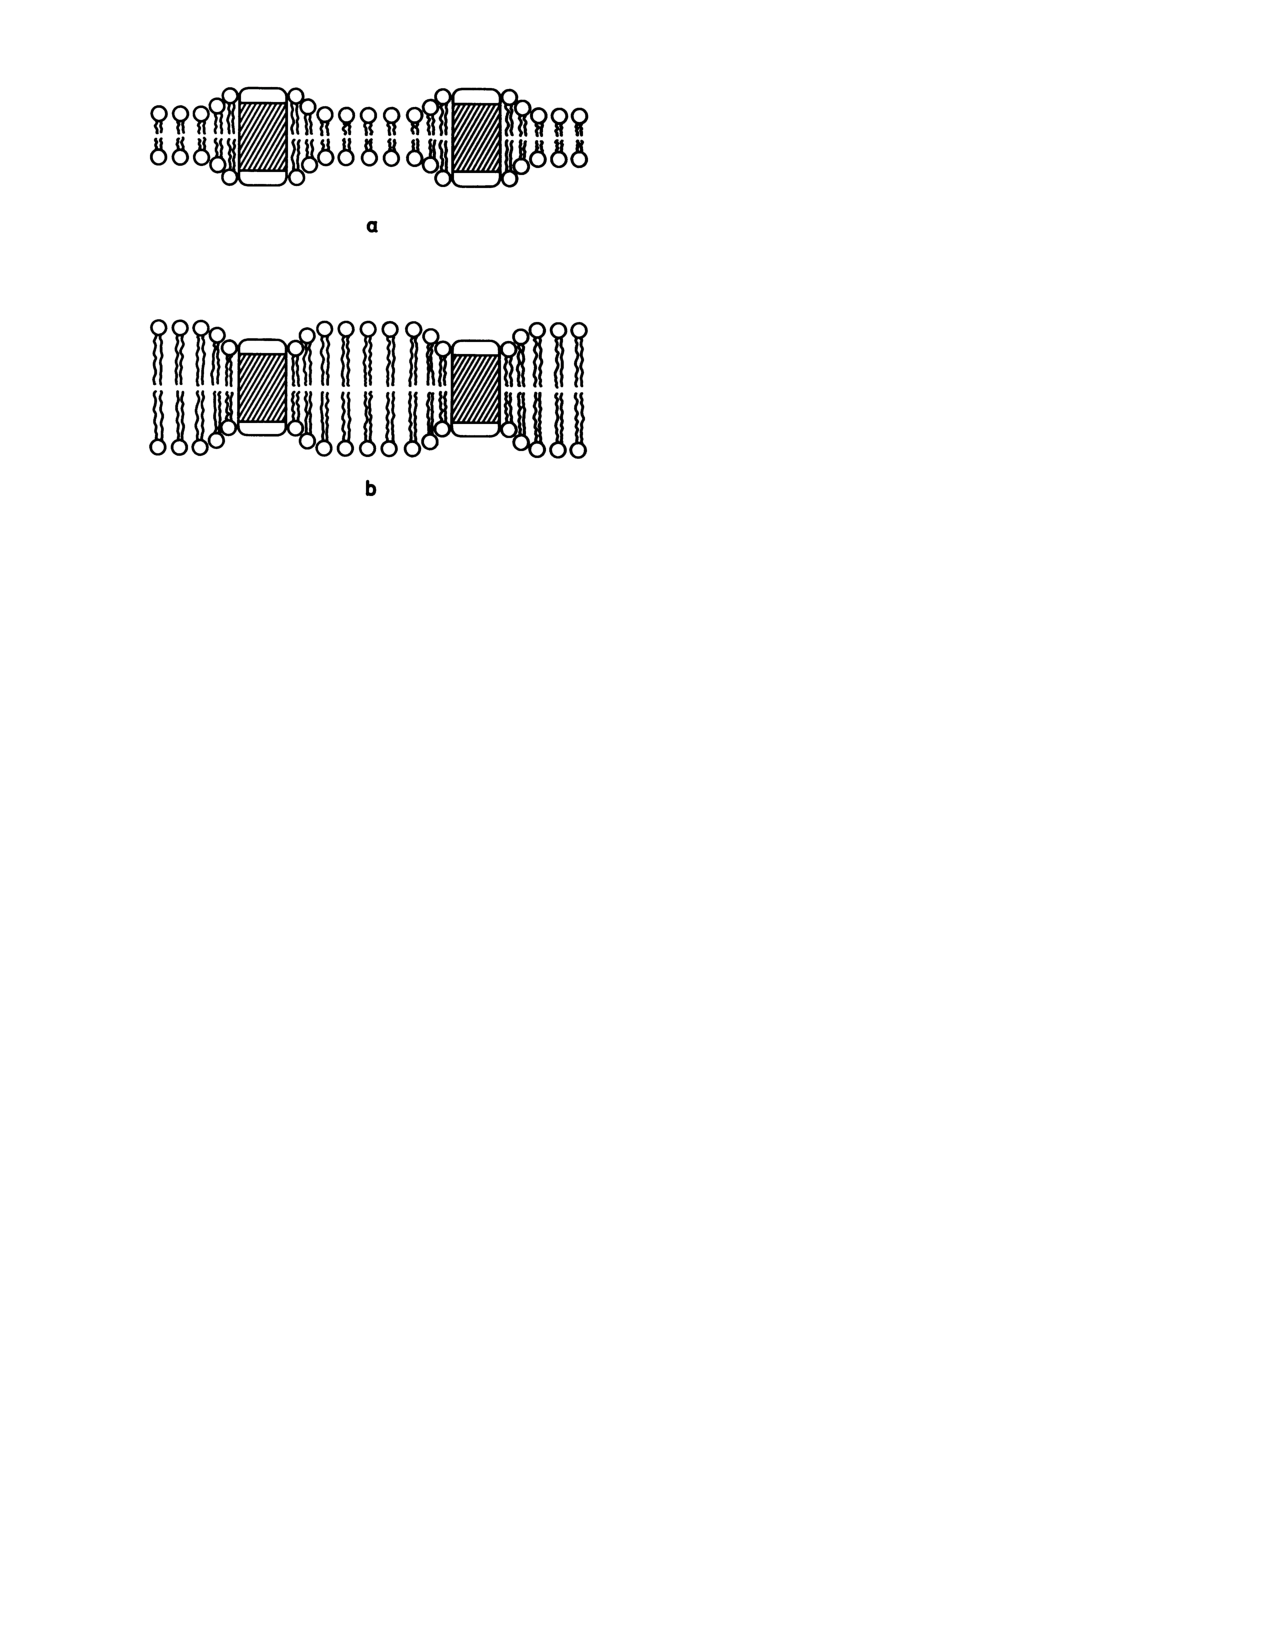
\includegraphics[width=4in]{\MemBio /Pics/BilayerPlusProtein}
\caption{
نقاشی از برش یک غشای لیپیدی که حاوی نوعی ناخالصی (مانند پروتئین یا پلی‌پپتید) است. ملکول‌های لیپید با دایره‌های سفید (سر آب‌دوست) و دم‌های آب‌گریز، و  ناخالصی‌ها به شکل مستطیل‌های دارای سر‌های آب‌دوست و ناحیه‌ی میانی هاشور خورده‌ی آب‌گریز نمایش داده شده‌است. اگر ناحیه‌ی آب‌گریز ناخالصی نسبت به غشا ضخیم‌تر (الف) یا نازک‌تر (ب) باشد، ضخامت غشا تحت تاثیر قرار می‌گیرد
\cite{Mouritsen1984}
.
}
\label{fig:BilayerPlusProtein}
\end{center}
\end{figure}





با وجود اینکه غشای لیپیدی به طور خود سامانده تشکیل می‌شود ولی علاوه بر ملکول‌های چربی پروتئین‌های زیادی نیز به غشا ساختار می‌بخشد
\cite{wikiCellMembrane}. غشاهایی هم می‌توان یافت که درصد پروتئین و کربوهیدارت در ساختار  آن به ترتیب بین ۱۸ تا ۷۵ درصد و  ۳ تا ۱۰ درصد باشد
\cite{MembraneProteins1972}. 
غشا از طریق این پروتئین‌ها به اجزای پیچیده‌تر داخل سلول (مانند اسکلت سلولی) متصل است. خاصیت تراوایی فوسفولیپید دو لایه و کانال‌های پروتئینی درون غشا، ارتباط سلول با محیط اطراف را کنترل و مدیریت می‌کند.  



\section{\label{sec:memBioSelfAssembily}
ساختارهای خودسامانده غشا
}
\setRL
%\pagenumbering{arabic} 
\section{
ساختارهای خودسامانده غشا
}
 
ملکول‌های لیپید یا چربی یکی از ۴ عناصری است که در کنار آمینو اسید‌ها، نوکلئیک اسید‌ها، و ملکول‌های قندی ساختار موجودات زنده را تشکیل می‌دهد که از این میان فقط لیپید‌ها پلیمر نیستند
\cite{Membraneasamatteroffat}. بیش از هزار نوع ملکول چربی در گونه‌های زیستی وجود دارد ولی ساختار کلی آنها بسیار مشابه است. در سلول‌ پستانداران بیشتر فسفولیپید و گلیسرول یافت می‌شود. ملکول‌ فوسفولیپید از یک سر آب‌دوست\LTRfootnote{hydrophilic}  
 و یک دُم آب‌گریز\LTRfootnote{hydrophobic}  
 ساخته شده‌است (شکل
\ref{fig:bilayer}). فرق بین ملکول‌های لیپید مختلف در ساختار شیمایی سر آب دوست و دُم آب‌گریز آنهاست. این ملکول‌ها در محلول‌های آبی
\textbf{بدون ایجاد پیوندها شیمیایی}، به طور خود سامانده\LTRfootnote{self-assembly}  
 تشکیل شده و ساختار‌های بسیار متنوعی دارند. اساس این ساختار‌ها کمینه کردن انرژی آزاد سیستم از طریق محافظت کردن دُم‌های آب‌گریز از آب است که با افزایش غلظت ملکول‌های لیپید ساختار‌های مختلفی تشکیل می‌شود
 (شکل
\ref{fig:bilayer}). برای مثال مایسِل‌ها\LTRfootnote{Micelle}
 در محلول‌های لیپدیدی با غلظت‌ پایین (ولی بالاتر از یک غلظت حدی) تشکیل می‌شود
 \cite{Lipowskyb1995ook}. در این ساختار انتهای تمام دُم‌های آب‌گریز در کنار هم قرار گرفته و سَر‌های آب‌دوست کُره تشکیل می‌دهند. هنگامی‌ که غلظت لیپید‌ها بیشتر شود یک تغییر حالت از مایسِل به ساختارهای دیگر مانند استوانه خواهیم دید. همچنین ساختار‌های ترکیبی نیز تشکیل می‌شود مانند در کنارهم قرار گرفتن استوانه‌ها در فاصله‌های
  $1-5nm$
طوری که محور استوانه‌ها بر روی شبکه‌ی شش ضلعی قرار می‌گیرد. 
 
 فرآوان‌ترین ساختار لیپید‌ها ساختار دو-لایه ‌است (شکل
 \ref{fig:bilayer}
 ب).  در ساختار‌های دو-لایه دُم‌های  آب‌گریز در مرکز لایه (به دور از آب) و سر آب‌دوست به سمت محلول جهت‌گیری می‌کند. از آنجایی که لبه‌های این سطوح شامل دُم‌های آب‌گریز است، به لحاظ انرژی هزینه‌بر است و به همین علت این سطوح هندسه‌های بسته تشکیل می‌دهند، مانند لیپوزم\LTRfootnote{Liposome}
 یا ساختار‌های ترکیبی مانند غشا‌هایی که از چندین دو-لایه تشکیل شده‌اند
\cite{LifeAsaMatterofFat2005}.

لازم به ذکر است که عوامل دیگری مانند دما و ترکیبات شیمیایی محلول بر نحوه‌ی تشکیل ساختار‌های لیپیدی تاثیر می‌گذارند. از آنجایی که دُم لیپید‌ها شکل ثابتی ندارد نمی‌توان حجم مشخصی برای این ملکول معین کرد. ولی تاثیر ترکیبات محلول، دما، و سایر عوامل موثر بر رفتار این ملکول را می‌توان با در نظر گرفتن حجم متوسط،
$v$، سهم سطح، 
$a$، و عمق اشغال شده ملکول درون ساختار،
$\ell$، مُدل کرد. این پارامتر‌ها با اندازه‌گیری روی اندازه‌ی سر دوقطبی، طول د‌ُم اسید چرب و حل‌شوندگی دُم در محلول تنظیم می‌شود
\cite{LifeAsaMatterofFat2005}. مثلا بالا رفتن دما  مُد‌های چرخشی زنجیر کربنی حول محور خود را افزاریش داده و در نتیجه سهم مساحت اشغالی ملکول بالا می‌رود
\cite{BiomembranesBook1989}. البته که این امر می‌تواند منجر به ذوب شدن غشا نیز شود
\cite{BioMemBook2007}.
 اسرائیلاچویلی\LTRfootnote{LiposomeIsraelachvili}
و همکارانش در یک مقاله‌ی معروف در سال ۱۹۷۶
\cite{Israelachvili1976}، با یک ضرب و تقسیم سر انگشتی تاثیر شکل ملکول‌های لیپیدی را توصیف می‌کنند. امکان قرار گرفتن یک ملکول لیپید در ساختاری مشخص با عدد بسته‌بندی یا پَکینگ\LTRfootnote{packing}
مشخص می‌شود:
\begin{equation}
%\begin\centering
P=\frac{v}{a\ell}
%\end\centering
\end{equation}
مثلا برای مایسِلی به شعاع، 
$R_m$، رابطه‌ی حجم، 
$v=\frac{1}{N}\frac{4\pi R_m^3}{3}$، و سطح 
$a=\frac{1}{N}4\pi R_m^2$ 
به این صورت تخمین زده می‌شود. در اینجا،
$N$، تعداد ملکول‌ها در ساختار مایسِل است. از آنجایی که شعاع مایسِل نمی‌تواند از طول دُم ملکول بزرگتر باشد (
$\ell\geq R_m$
):
\begin{equation}
%\begin\centering
P_m=\frac{v}{a\ell}=\frac{\frac{1}{N}\frac{4\pi R_m^3}{3}}{\frac{1}{N}4\pi R_m^2\ell}=\frac{1}{3}\frac{R_m}{\ell}\leq\frac{1}{3}
%\end\centering
\end{equation}
پس عدد پَکینگ باید کمتر از 
$\frac{1}{3}$
باشد تا ساختار‌‌های مایسِل پایدار داشته باشیم. این محاسبات برای  ساختارهای استوانه‌ای به شعاع، 
$R_c$
، و طول بلند، 
$L\gg R_c$
به این شکل انجام می‌شود،
\begin{equation}
%\begin\centering
P_c=\frac{v}{a\ell}=\frac{\frac{1}{N}\pi LR_c^2}{\frac{1}{N}2\pi LR_c\ell}=\frac{1}{2}\frac{R_c}{\ell}\leq\frac{1}{2}
%\end\centering
\end{equation}
در نتیجه ساختار استوانه‌ای پایدار در عدد پَکینگ 
$\frac{1}{3}<P<\frac{1}{2}$
ایجاد می‌شود. با تکرار محاسبات مشابه عدد عدد پَکینگ برای ساختار‌های دو لایه
$\frac{1}{2}<P<1$
تخمین زده می‌شود. لیپید‌هایی که از غشاهای زیستی استخراج می‌شود بیشتر 
$P>1$
دارند، در نتیجه‌ شکل کلی آن‌ها شبیه به یک مخروط وارونه است. در نتیجه دو-لایه‌هایی که فقط از ملکول‌های لیپید زیستی ساخته شده باشد تنش‌ها خمشی زیادی خواهد داشت
\cite{Mouritsen2011,Membraneasamatteroffat}. این تنش‌ها با اضافه شدن پروتئین‌ها و تشکیل حباب‌های کوچک (هم رو به داخل
\LTRfootnote{endocytosis}
  هم رو به بیرون
 \LTRfootnote{exocytosis}) بر روی غشای سلول آزاد می‌شود.



\begin{figure}[h]
\begin{center}
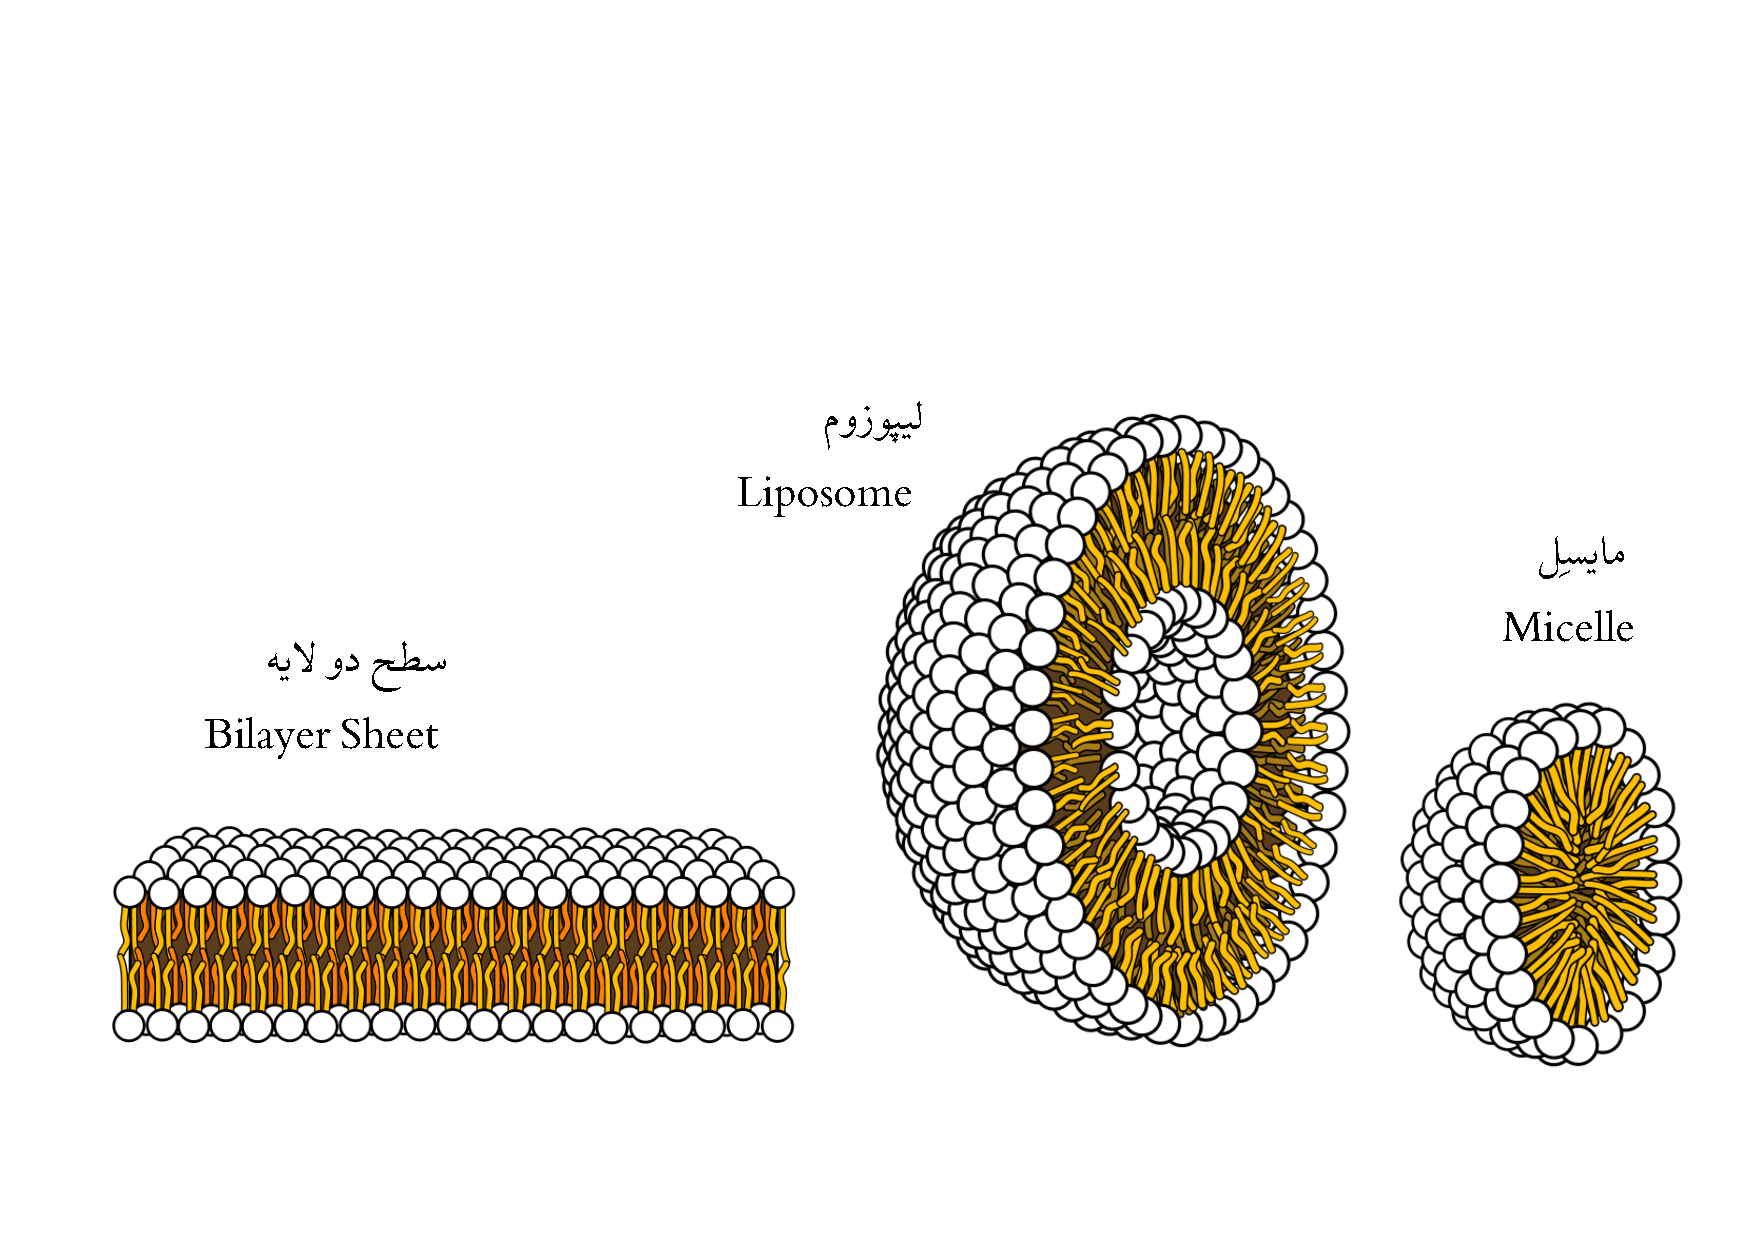
\includegraphics[width=4in]{\MemBio /Pics/Bilayer}
\caption{
الف) ساختار شیمیایی یک ملکول فوسفولیپید. سر آب‌دوست (دایره‌ی آبی) و  انتهای آب‌گریز مشخص شده است. ب) ساختار‌های معمول ملکول‌های چربی در آب. به ترتیب از چپ به راست، ساختار سطوح بزرگ دو-لایه، کُره‌های دو-لایه (لیپوزوم)، و کره‌های کوچک تک لایه، مایسِل.
}
\label{fig:bilayer}
\end{center}
\end{figure}




\begin{figure}[h]
\begin{center}
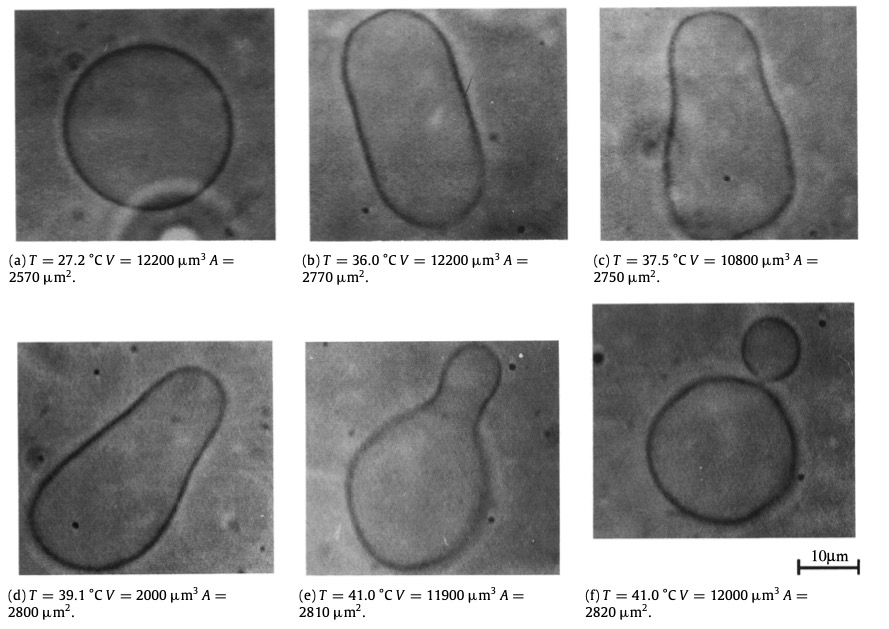
\includegraphics[width=4in]{\MemBio /Pics/GUVTempChange}
\caption{
تغییر ساختار یک غشای غول ‌آسا به علت تغییر دما از ۲۷/۲ تا ۴۱ درجه‌ی سانتیگراد. در دمای ۳۶ درجه حالت بیضی شکل، بالاتر از دمای ۳۶ شکل گلابی، و با ماندن در دمای ۴۱ درجه یک حباب بر روی آن جدا شده.
}
\label{fig:GUVTempChange}
\end{center}
\end{figure}






با وجود پیچیدگی‌ که در غشای سلول‌های زیستی هست، آن‌ها نیز باید از قوانین فیزیکی حاکم بر اجسام بی‌جان پیروی کنند. از طرفی غشا‌ها بیشتر دارای ساختارهای متنوع و خاص هستند تا ساختارهای مشترک که بتوان عمومیت داد
\cite{NelsonBook2004}.
ولی می‌توان خواص فیزیکی غشاها را با قوانین ترمودینامیک به صورت درشت دانه مدل کرد و رفتار‌ آن‌ها را در طیفی از هندسه‌ها و مقیاس‌ها مشخص کرد
\cite{Seifert1997}.
 مثلا انرژی مشخصه اندازه‌گیری شده برای تجمع واحد‌های تشکیل‌ دهنده‌ی غشاهای زیستی یک مرتبه‌ی بزرگی از انرژی گرمایی محیط 
$k_BT$
بیشتر گزارش شده. در اینجا، 
$k_B$،
ثابت بُلتسمَن و 
$T\approx300K$،
دمای محیط است. در نتیجه ساختار غشاهای زیستی در مقابل افت و خیز گرمایی در نزدیکی دماهای فیزیولوژیکی پایدار است. همچنین آنقدر نرم  هستند که توسط فرآیندهای زیستی مانند اتصال پروتئین‌ها
\cite{NelsonBook2004,Seifert1997,Deserno2015}،
ATP
هیدرولسیز
\LTRfootnote{ATP hydrolysis}
\cite{Boyle2008Biology,Lipowskyb1995ook}
تغییر شکل می‌دهند.
یکی از خواص مهم و جالب غشاها مقاومت خیلی کمِ خم شدنِ آن‌ها تحت نیروی خارجی است. این پدیده، افت و خیز دیواره‌ی سلولی، با میکروسکوپ نوری به راحتی قابل مشاهده است
\cite{NelsonBook2004}.
جذابیت دیگر غشا‌ها برای فیزیکدان‌ها ضخامت خیلی کم آن‌هاست که در نتیجه می‌توان آن را با یک صفحه‌ی ۲ بعدی مدل‌سازی کرد و ابعاد مسئله‌ را کاهش داد
\cite{Seifert1997,Deserno2015}.
درنتیجه‌ی مطالعه‌ی غشاها با استفاده از این نوع ساده‌سازی و مدل سازی می‌توانیم  رفتار آن‌ها را در مقیاس‌های مختلف پیش‌بینی کرده و نقش‌ آن‌ها را در فرآیند‌های زیستی توصیف کنیم.



محققان با مطالعه‌ی غشا‌های غول‌آسا
\LTRfootnote{Giant Unilamellar vesicle}  
 یا 
 GUV اطلاعات  زیادی راجع به ساماندهی غشاهای چربی جمع‌آوری کرده‌اند. این غشا‌ها را معمولا می‌توان با  مخلوط کردن\LTRfootnote{mixing}  
 غشا‌ و ترکیب‌های چربی در آزمایشگاه ساخت
 \cite{GUVmaking2009}
و اندازه‌ی آن می‌تواند از چند میلی‌متر تا چند میکرون  باشد. 
GUV نسبت به تغییرات ترمودینامیکی محیط واکنش‌های بسیار جالبی نشان می‌دهد. برای مثال شکل
\ref{fig:GUVTempChange}
ایجاد یک حباب کوچک بر روی یک GUV را با تغییر دمای محیط از ۲۷ تا ۴۱ درجه در قالب ۶ سری عکس پشت سر هم نشان می‌دهد
\cite{MemReviewRamakrishnan2014}.
 
\begin{figure}[h]
\begin{center}
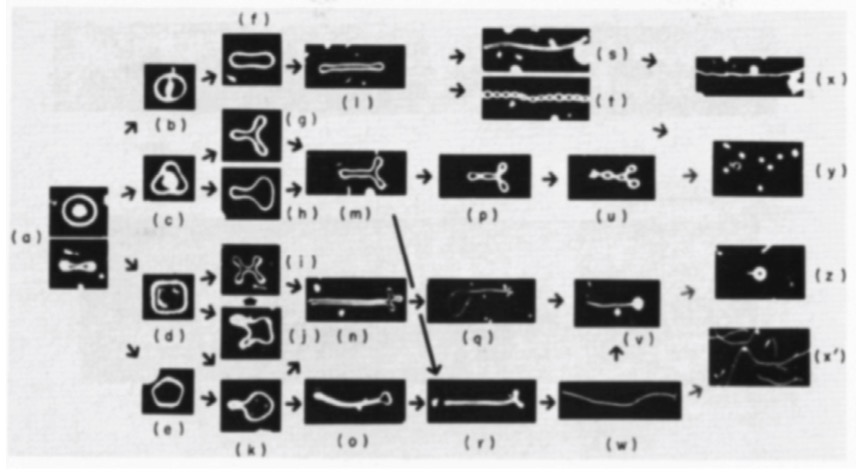
\includegraphics[width=4in]{\MemBio /Pics/GUVPresChange}
\caption{
مسیر‌های مختلفی که یک غشای غول آسای آب نباتی شکل (ستون سمت چپ، زاویه‌ی دوربین از بالا و کنار) که بر اثر تغییر غلظت نمک محیط طی می‌کند تا به شکل خیلی کشیده (ستون سمت راست) در بیاید، را نشان می‌دهد.
}
\label{fig:GUVPresChange}
\end{center}
\end{figure}

GUV همچنین نسبت به تغییرات فشار اسمزی محیط نیز واکنش نشان می‌دهد. مثلا در شکل 
\ref{fig:GUVPresChange}
می‌بینیم که با تغییر غلظت نمک در محیط یک غشایِ لیپیدیِ دارای کلسترول، از شکل اولیه آب نباتیِ\LTRfootnote{biconcave}  
شبیه‌ به گلبول قرمز به حالت کشیده و لوله‌ای در می‌آید. در شکل 
\ref{fig:GUVPresChange}
ساختار‌های هندسی میاینی (و در مواردی ناپایدار) مختلفی که غشا طی می‌کند تا از هندسه‌های سمت چپ به هندسه‌های سمت راست برسد، را می‌توان مشاهده کرد.
  
 
 
 
 
 
 
 
 
 
 

\section{\label{sec:memBioGUVs}
غشاهای غول‌آسا
}
%\setRL
%\pagenumbering{arabic} 

\begin{figure}[t]
\begin{center}
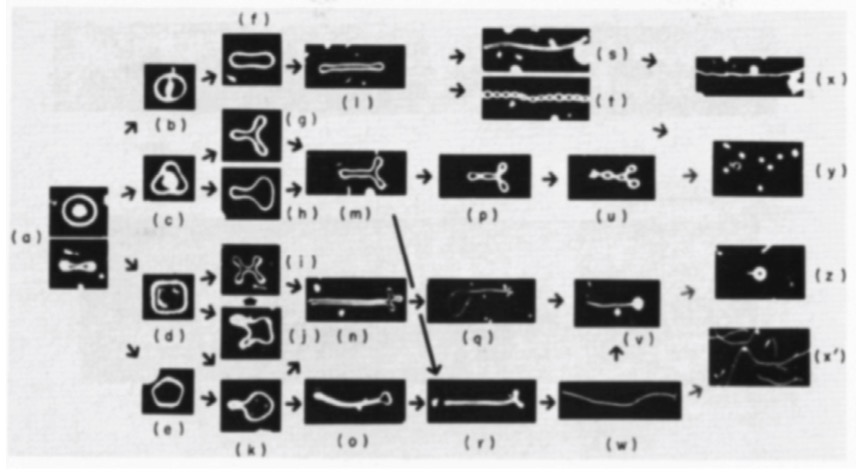
\includegraphics[width=\columnwidth]{\MemBio /Pics/GUVPresChange}
\caption{
مسیر‌های مختلفی که یک غشای غول آسای آب نباتی شکل (ستون سمت چپ، زاویه‌ی دوربین از بالا و کنار) که بر اثر تغییر غلظت نمک محیط طی می‌کند تا به شکل خیلی کشیده (ستون سمت راست) در بیاید.
}
\label{fig:GUVPresChange}
\end{center}
\end{figure}

\begin{figure}[t]
\begin{center}
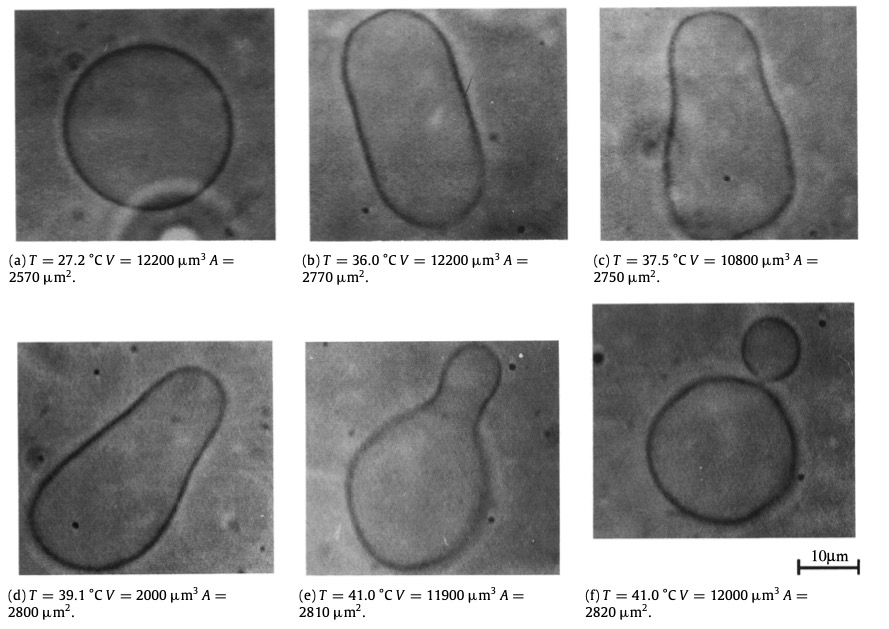
\includegraphics[width=\columnwidth]{\MemBio /Pics/GUVTempChange}
\caption{
تغییر ساختار یک غشای غول ‌آسا به علت تغییر دما از ۲۷/۲ تا ۴۱ درجه‌ی سانتیگراد. در دمای ۳۶ درجه حالت بیضی شکل، بالاتر از دمای ۳۶ شکل گلابی، و با ماندن در دمای ۴۱ درجه یک حباب بر روی آن جدا شده‌است.
}
\label{fig:GUVTempChange}
\end{center}
\end{figure}


محققان با مطالعه‌ی غشا‌های غول‌آسا
\LTRfootnote{Giant Unilamellar vesicle}  
 یا 
 GUV اطلاعات  زیادی راجع به ساماندهی غشاهای چربی جمع‌آوری کرده‌اند. این غشا‌ها را معمولا می‌توان با  مخلوط کردن\LTRfootnote{mixing}  
 غشا‌ و ترکیب‌های چربی در آزمایشگاه ساخت
 \cite{GUVmaking2009}
و اندازه‌ی آن می‌تواند از چند میکرون تا چند میلی‌متر   باشد.
این غشاها از یک دولایه‌ی خیلی ساده لیپیدی تشکیل شده‌اند و در نتیجه‌ ضخامت‌ آن‌ها بین ۴ -۵ میلی‌متر است (دو برابر اندازه‌ی یک مولکول لیپید). غشاهای زیستی ساختار پیچیده‌تری دارند ولی در اصل تمام‌ غشاهای زیستی بر بستر یک ساختار دو لایه‌ی لیپیدی بنا شده‌اند و در نتیجه می‌توان خواص مشترک زیادی میان غشا‌های غول‌آسا و غشاهای زیستی پیدا کرد.
غشاهای دولایه، مرز مشخصی میان شاره‌‌‌ای که درون خود بسته‌بندی کرده‌اند و شاره‌ای که در محیط اطراف است تشکیل می‌دهند. ساختار غشا نسبت به مولکول‌های کوچک غیر باردار مانند 
$H_2O$، 
$O_2$،
و 
$CO_2$
و همچنین
$H_3O^+$
و
$OH^-$
تراوا است ولی نسبت به مولکول‌های درشت‌ترِ حلال در آب مانند گلوکز\LTRfootnote{glucose}
و منوساکارید‌ها\LTRfootnote{monosaccharid}
 تراوا نیست. در نتیجه‌ حضور چنین مولکول‌هایی در محیط، فشار اسمزی بر غشا وارد خواهد کرد. فشار اسمزی به اختلاف غلظت مولکول‌های درون و خارج از غشا بستگی دارد و باعث جابجایی آب داخل غشا می‌شود. در صورتی که غلظت حل شونده در خارج از غشا بیشتر باشد، شبیه به یک پمپ، آب از درون غشا خارج می‌شود و نسبت حجم به سطح غشا را تغییر می‌دهد. برعکس، در صورتی که غلظت مولکول‌ها درون غشا بیشتر از محیط باشد، آب از محیط به درون غشا پمپ می‌شود. تغییر شکل غشا در این صورت تا جایی ادامه پیدا می‌کند که شکل یک کُره به خود بگیرد. اگر همچنان آب به داخل غشا منتقل شود کمی سطح غشا کشیده می‌شود (کُره رشد می‌کند) تا جایی که تحمل کشش غشا تمام شود و غشا پاره خواهد شد.





همانطور که در شکل 
\ref{fig:GUVPresChange}
نشان داده‌ شده‌است، با تغییر غلظت نمک در محیط یک غشایِ لیپیدیِ دارای کلسترول، از شکل اولیه آب نباتیِ\LTRfootnote{biconcave}  
شبیه‌ به گلبول قرمز به حالت کشیده و لوله‌ای در می‌آید. در شکل 
\ref{fig:GUVPresChange}
ساختار‌های هندسی میاینی (و در مواردی ناپایدار) مختلفی که غشا طی می‌کند تا از هندسه‌های سمت چپ به هندسه‌های سمت راست برسد، را می‌توان مشاهده کرد.
GUV نسبت به تغییرات ترمودینامیکی محیط واکنش‌های بسیار جالبی نشان می‌دهد. برای مثال شکل
\ref{fig:GUVTempChange}
ایجاد یک حباب کوچک بر روی یک GUV را با تغییر دمای محیط از ۲۷ تا ۴۱ درجه در قالب ۶ سری عکس پشت سر هم نشان می‌دهد
\cite{MemReviewRamakrishnan2014}.



 

 
 
 
 
 
 
 
 
 
 
 
 

\section{\label{sec:memBioFluidity}
خواص سیال‌گون غشا
}
\setRL
%\pagenumbering{arabic} 
\section{
خواص سیال‌گون غشا
}

دیگر خاصیت مشترک میان تمام غشا‌ها این است که به علت سرعت بالای پخش ملکول‌ها بر روی سطح آن، حالت سیال بودن خود را حفظ می‌کند. سیال بودن غشا تقریبا از ده‌ی ۱۹۷۰ به بعد توسط عموم پذیرفته شد. در آن زمان آزمایش‌هایی به طور همزمان و مستقل شواهدی ارائه دادند که خاصیت سیال‌گون غشا را نشان می‌داد. اولین مشاهده در این تحقیقات مربوط به اندازه‌گیری سرعت پخش ملکول‌های لیپیدی  با برچسب اسپینی
\LTRfootnote{spin-labelled lipids}
\cite{Kornberg1971DiffusionPhospholipids, Devaux1972LateralDiffusion}
و ملکول‌های استروید
\LTRfootnote{steroids}  
\cite{Sackmann1972, Traeubl1972}
بر سطح غشا بود که حدود 
$1 \mu m^2\cdot sec^{-1}$
اندازه‌گیری شد. روش‌های جدید اندازه‌گیری  حرکت ملکول‌های فلورسانت
\LTRfootnote{fluorescence recovery after photobleaching (FRAP)}  
\cite{almeida1992lateral }
و همچنین روش‌های شناسایی تک ذره‌ای 
\LTRfootnote{single particle tracking}  
\cite{Sako1994, Saxton1997, Fujiwara2002, Kusumi2005}
این ضریب پخش را در مورد غشاها تایید می‌کنند.

دومین سر آزمایش‌هایی که ماهیت سیال‌گون غشا را تایید کرد  مطالعات بر روی نحوه‌ی تغییر شکل گلبول‌های قرمز 
\cite{Canham1970, Evans1974}
و غشاهای لیپیدی
\cite{Helfrich1973, Helfrich1976}
انجام شده ماهیت سیال‌گونه‌ی غشا را نیز تایید می‌کند. در اثر تغییر شکل، خمش سطح غشا  به طور پیوسته و بدون شکستگی تغییر می‌کند و در صورتی که جنس غشا جامد و یا پلیمری باشد چنین تغییر شکلی امکان پذیر نخواهد بود. به طور مشخص این نوع تغییر شکل زمانی مشاهده می‌شود که حباب‌های جانبی بر روی سطح غشا تشکیل می‌شود (شکل 
\ref{fig:budding}
).

\begin{figure}[h]
\begin{center}
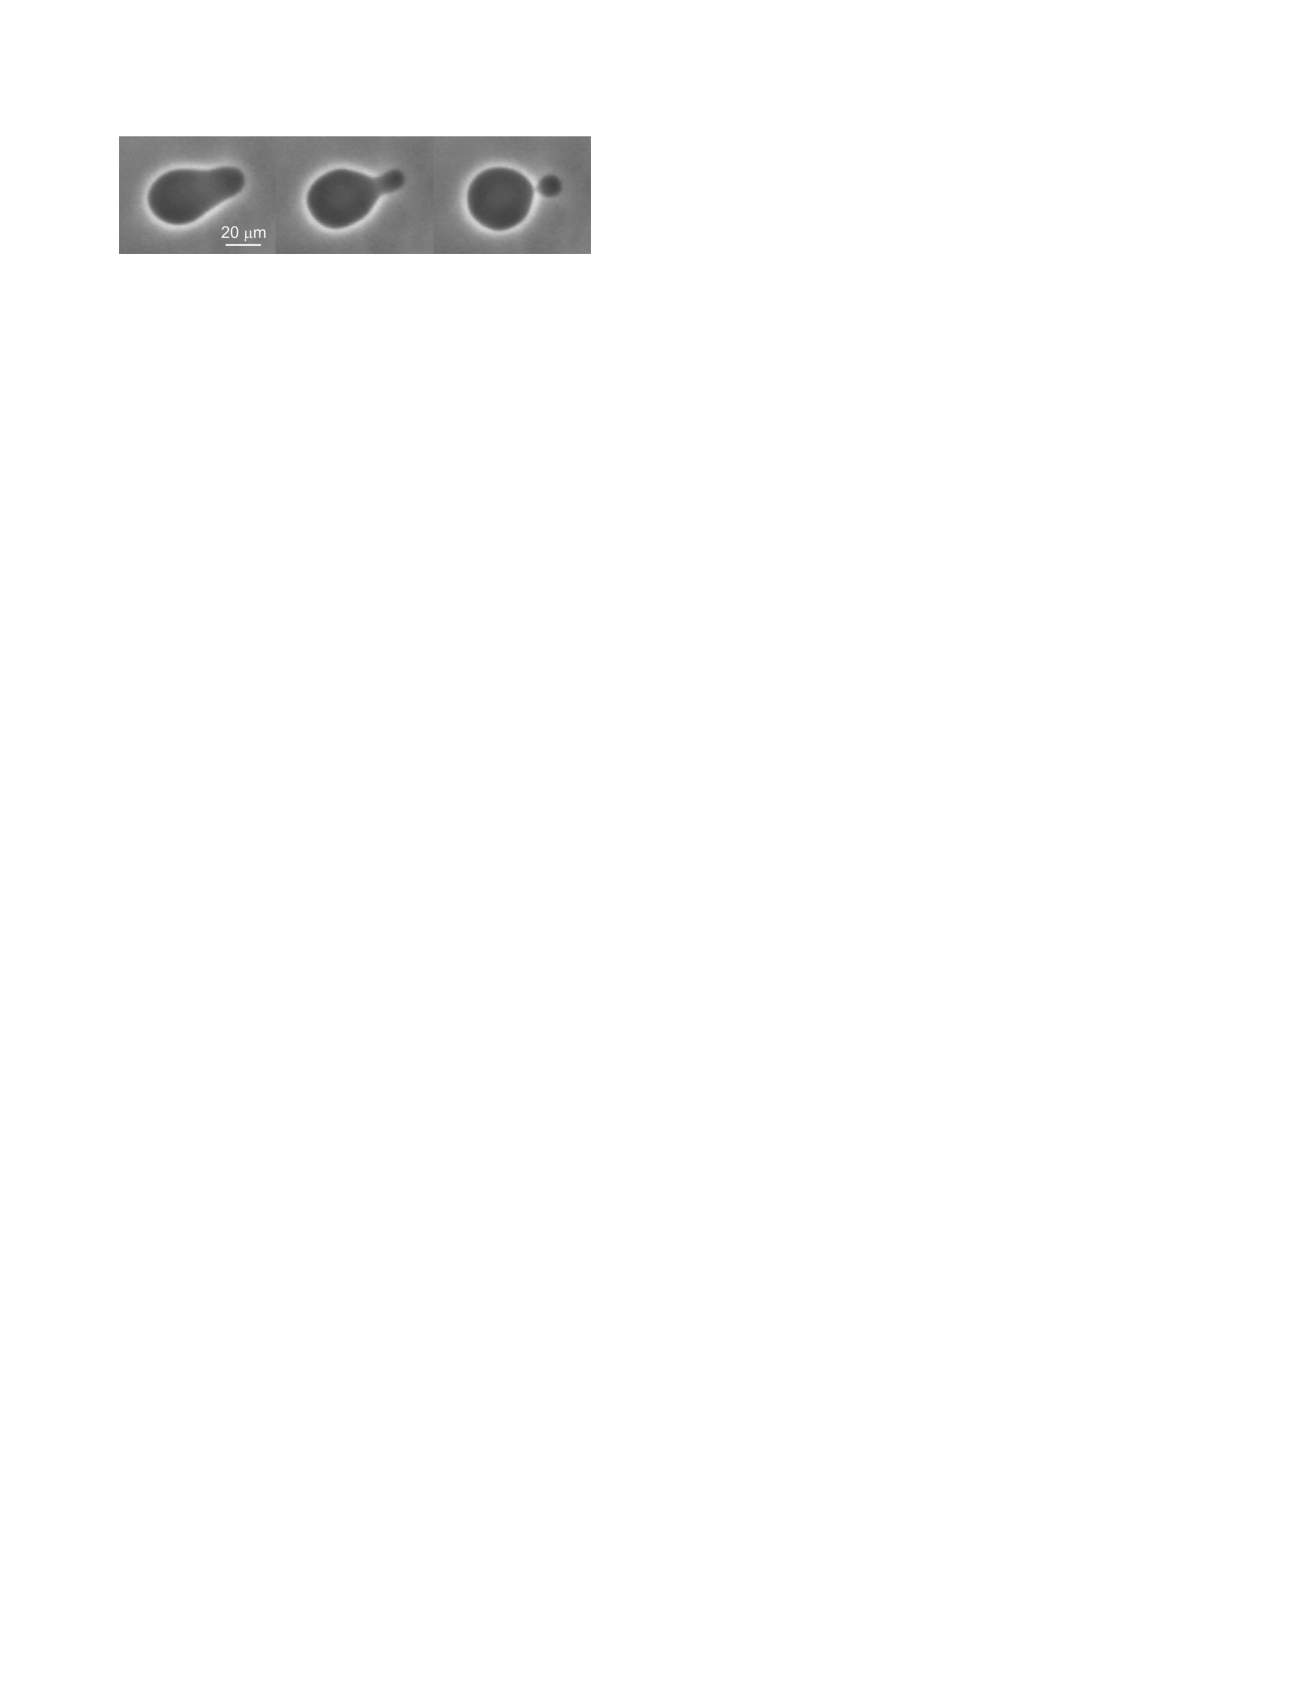
\includegraphics[width=6in]{\MemBio /Pics/budding.pdf}
\caption{
تشکیل یک غشای حبابی بر سطح یک غشای غول‌آسا در تصویربرداری میکروسکوپی اختلاف فازی. این حباب ظرف ۵ ثانیه تشکیل  شده که نشان از جنس سیال‌گون غشا است.
\cite{Dimova2006} 
}
\label{fig:budding}
\end{center}
\end{figure}

این نوع جوانه‌زدن
\LTRfootnote{budding}  
یکی از مهم‌ترین ساز‌ و کار‌های مبادله‌ی ملکول با محیط در سلول‌های زیستی‌ است. در یک سری از فرآیند‌های زیستی سلول پروتئین‌ها رو به سطح داخلی غشا منتقل می‌کند و با ایجاد جوانه می‌تواند ملکول‌های خود را به محیط صادر کند. عکس این فرآیند هم انجام می‌شود که بر اثر آن سلول اطلاعاتی از سلول‌های حاضر در محیط اطراف خود دریافت می‌کند.








\section{\label{sec:nuclearenvelope}
بسته‌ی هسته‌ی سلول
}
%\setRL
%\pagenumbering{arabic} 


\begin{figure}[t]
\begin{center}
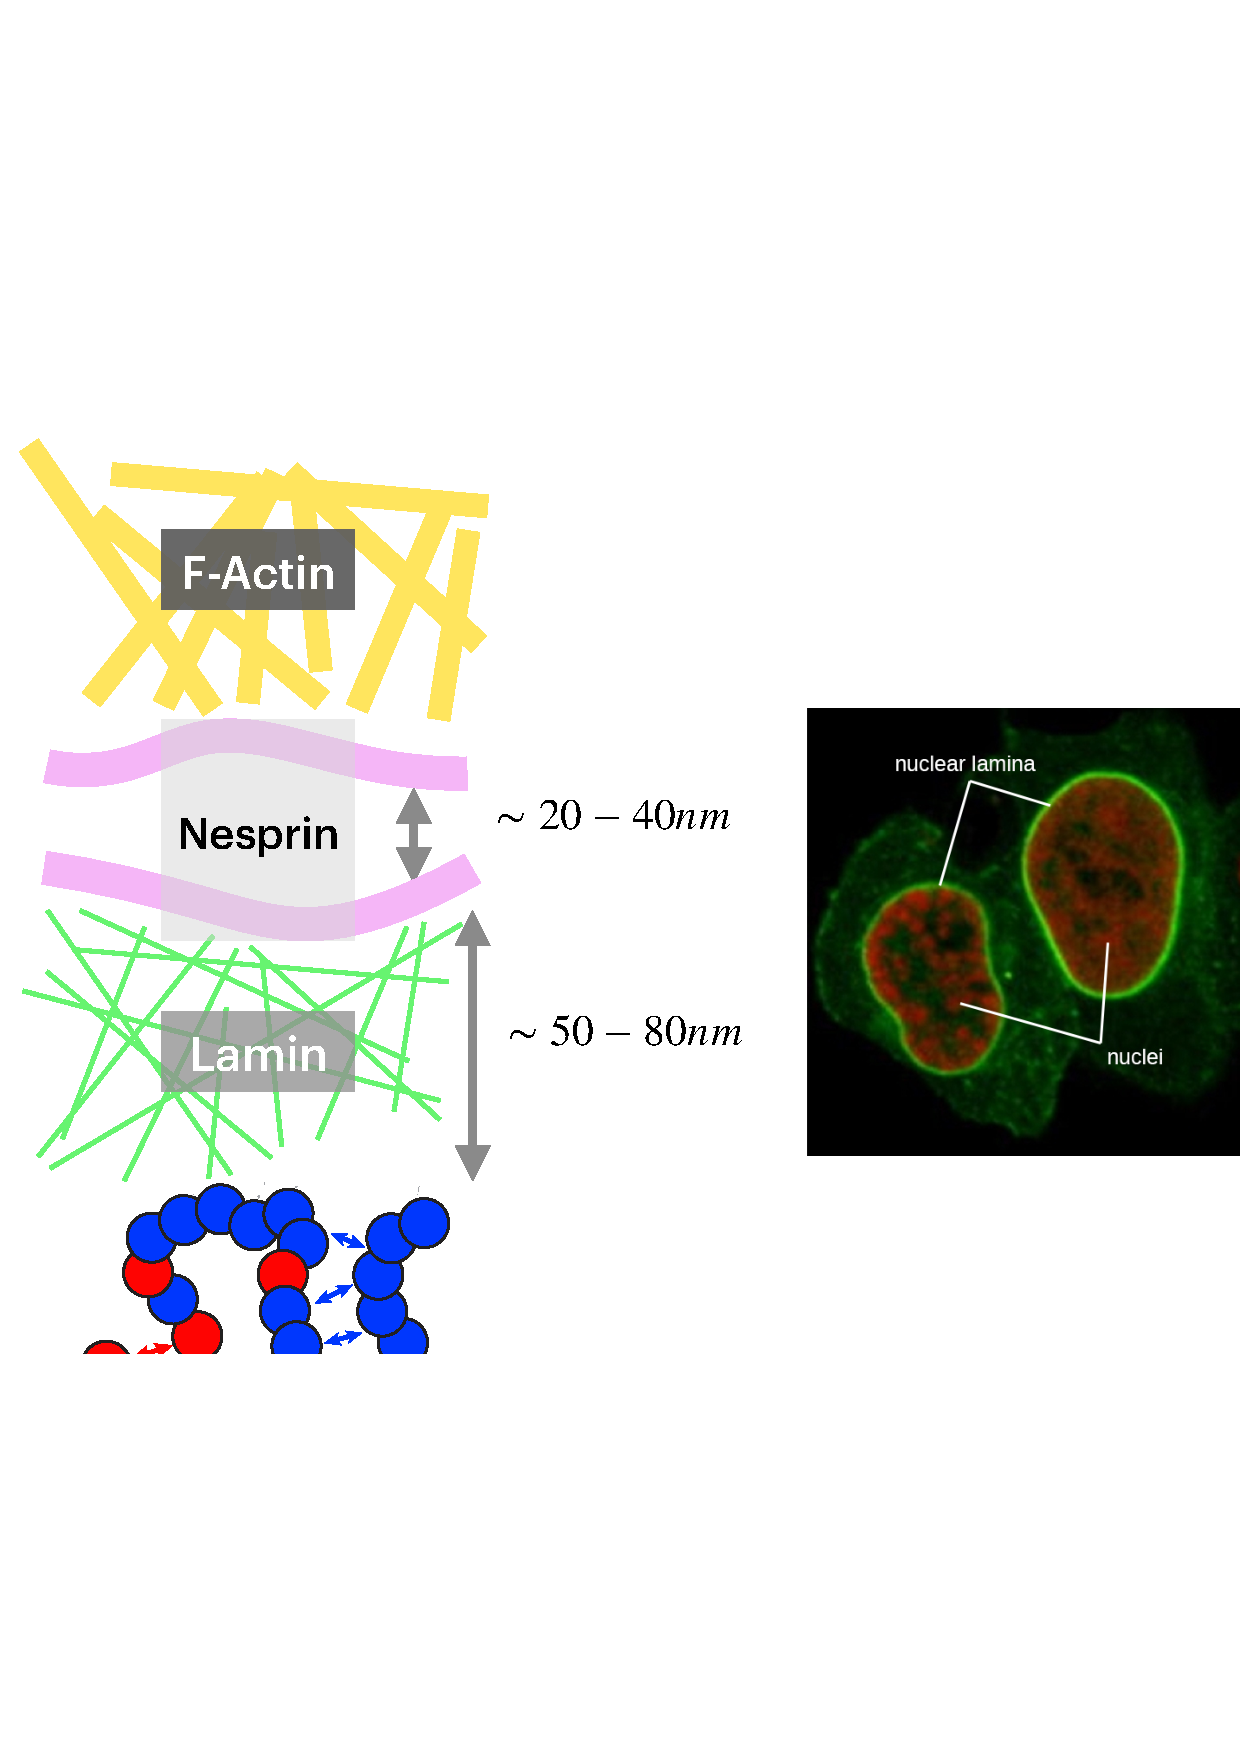
\includegraphics[width=6in]{\MemBio /Pics/NuclearEnvelope}
\caption{
عکس سمت راست، تصویر رنگ آمیزی شده‌ی هسته. لایه‌ی لمینا با رنگ سبز روشن، و کروماتین‌های درون هسته با رنگ قرمز نمایش داده‌ شده‌است. شکل سمت چپ، نقاشی ساختار بسته‌ی هسته است. از بالا به پایین: شبکه‌ی اکتین (زرد) که با پروتئین‌های نسپرین به غشای دولایه‌ی بیرونی (نوار صورتی) متصل شده‌است. غشای داخلی نیز به کمک همین پروتئین به لایه‌ی لمینا (سبز) متصل شده‌است. فضای میان غشای داخلی و خارجی از ۲۰ تا ۴۰ نانومتر تغییر می‌کند. ضخامت لمینا نیز بین ۵۰ تا ۸۰ نانومتر است. کروماتین‌های درون هسته (دایره‌های آبی و قرمز) می‌توانند با لایه‌ی لمینا اتصالاتی برقرار می‌کند. 
}
\label{fig:nuclearenvelope}
\end{center}
\end{figure}


غشای هسته یا نام رایج آن، بسته‌ی هسته\LTRfootnote{nuclear envelope}
ساختاری متفاوت نسبت به غشای سلول دارد. در خارج و اطراف هسته، ساختارهای زیادی وجود دارد، مانند شبکه‌ی اکتین\LTRfootnote{actin network}
 و میکروتیوبول‌ها\LTRfootnote{microtubules}.
 هسته‌ی سلول از طریق بسته‌ی هسته با تمامی‌ ارگان‌های لازم در ارتباط است.

در شکل 
\ref{fig:nuclearenvelope}
نقاشی از ساختار کلی بسته‌ی هسته را می‌بینیم. از بالا به پایین، خطوط زرد رنگ نماینده‌ی شبکه‌ی پروتئینی اکتین است. این شبکه از طریق پروتئین‌هایی به نام نسپرین\LTRfootnote{nesprin},
 که روی بسته‌ی هسته وجود دارند، به بسته‌ی هسته متصل است و نقش پُلی برای انتقال نیرو‌های خارج از سلول به هسته‌ی سلول را ایفا می‌کند
\cite{Lammerding2011}. 
بسته‌ی هسته از دو عدد غشای لیپیدی دو لایه (نوارهای صورتی) با نام غشای بیرونی و غشای داخلی تشکیل شده. ضخامت فضای بین دو غشا از ۲۰ تا ۴۰ نانومتر تغییر می‌کند. میان دو غشا را مایعی شبیه به سیتوپلاسم و شبکه‌ پروتئینی مورد نیاز برای انتقال مواد بین هسته و سلول، پر می‌کند. پروتئین‌های نسپرین  در غشای داخلی هم حضور دارد و این غشا را به شبکه‌ی پروتئینی لمینا\LTRfootnote{lamina}
(شکل
\ref{fig:nuclearenvelope}
نقاشی سمت چپ، خطوط سبز‌ رنگ) متصل می‌کند. لمینا‌ شبکه‌ای است به ضخامت حدود ۵۰ تا ۸۰ نانومتر که تمام سطح غشای داخلی را پوشانده است. در تصویر سمت راست شکل 
\ref{fig:nuclearenvelope}
با استفاده از روش‌های رنگ آمیزی میکروسکوپی، لایه‌ی لمینا را به رنگ سبز روشن می‌بینیم که کروماتین‌های (قرمز) درون هسته را محصور کرده‌اند. لمینا خاصیت الاستیکی دارد و تقریبا تمام ویژگی الاستیک بسته‌ی هسته به علت وجود این بخش است
\cite{Steensel2017wd}.
مدول الاستیک شبکه‌ی اکتین تقریبا ۵۰۰ پاسکال، و مدول الاستیک هسته‌ی سلول زمانی که درون سلول قرار دارد، ۵ هزار پاسکال و هنگامی ‌که از سلول خارج شده باشد، ۸ هزار پاسکال اندازه‌گیری شده‌است
\cite{Dahl2004, CAILLE2002177}.







